%% name: 023
\documentclass[border=1pt]{standalone}
\usepackage{xcolor}
\usepackage{amsmath}
\usepackage{tikz}
\begin{document}
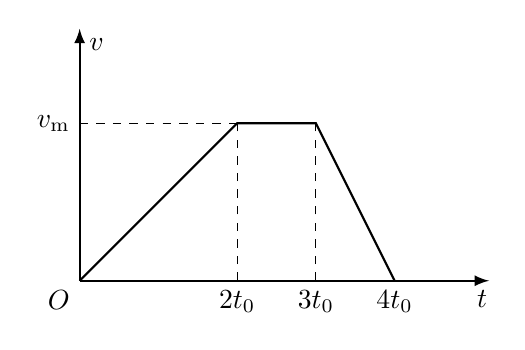
\begin{tikzpicture}[>=latex]
% ===== 坐标轴 =====
\draw[->, thick] (0,0) -- (5.2,0);
\draw[->, thick] (0,0) -- (0,3.2);

% ===== 轴标签 =====
\node[below left] at (0,0) {$O$};
\node[below left] at (5.3,0) {$t$};
\node[below right] at (0,3.2) {$v$};

% ===== 刻度标签 =====
\node[below] at (2,0) {$2t_0$};
\node[below] at (3,0) {$3t_0$};
\node[below] at (4,0) {$4t_0$};
\node[left] at (0,2) {$v_{\mathrm{m}}$};

% ===== 虚线辅助线 =====
\draw[dashed, thin] (0,2) -- (2,2);       % v_m 水平虚线
\draw[dashed, thin] (2,0) -- (2,2);       % 2t_0 竖直虚线
\draw[dashed, thin] (3,0) -- (3,2);       % 3t_0 竖直虚线

% ===== 主图线（梯形） =====
\draw[thick] (0,0) -- (2,2) -- (3,2) -- (4,0);
\end{tikzpicture}
\end{document}